\section{Confidential Computing}
\label{sec:confidential-computing}

Moving on from the traditional distributed computing model, this section gives
an overview of the current state of confidential computing.

Data can be in three distinct states: ``at rest'', ``in transit'', and ``in
use''. These three states describe data that are stored in persistent storage,
traversing a network, and data that is currently being processed. While
technologies protecting data ``at rest'' and ``in transit'' are commonly used
today, there are not many methods to protect data ``in use''.

Confidential computing provides hardware-based primitives that allow the
creation of trusted execution environments (TEEs). These TEEs have certain
properties that protect data that is currently in use by applications from
unauthorized access.

\subsection{Trusted Execution Environments (TEEs)}
\label{sec:tee}

\subsubsection{Properties}

There are different definitions of a trusted execution environment (TEE) with
varying properties. The three main properties defined by the
\textit{Confidential Computing Consortium} \cite{ccc2022technicalanalysis} are:

\begin{description}
  \item[Data confidentiality]
    Prevent unauthorized entities to view data that is in use within a TEE.
  \item[Data integrity]
    Prevent unauthorized entities to add, remove, or change data while it is in
    use within a TEE.
  \item[Code integrity]
    Prevent unauthorized entities to add, remove, or change code executing in
    the TEE.
\end{description}

Besides ensuring the confidentiality of data, code integrity is also critical
for the confidentiality of data. Even if data confidentiality is implemented
correctly, executing compromised code inside TEEs can also lead to leakage of
confidential data.

Provided that the application code implements the computation correctly, data
and code integrity ensure that neither the data nor the application have been
modified, allowing clients to trust the results of the computations run inside
TEEs.

As TEE technologies widely differ in their implementations, this thesis will
treat the hardware and software components that create and protect TEEs as a
single platform, which consists of all hardware and software components involved
and refer to it as the ``TEE platform''.

Besides the three core properties TEE platforms also often provide mechanisms
that allow the integration of a remote attestation process (see Section
\ref{sec:remote-attestation}), enabling clients to assess the trustworthiness of
TEEs provided by an untrusted party. These technologies generally produce
evidence about the authenticity and integrity of both the TEE platform and
specific TEEs.

\subsubsection{Hardware Support}

The security of a software layer can only be as strong as the layers below it.
This is why an ideal security solution acts from the lowest layer possible. By
providing security through the lowest layer -- the hardware -- it is possible to
remove almost all software components between the hardware and the TEE from the
list of trusted components, including system software such as the operating
systems and hypervisors. The only components that need to be trusted are the
components of the TEE platform.

Today most TEE implementations still rely on firmware components that are part
of the TEE platform. This allows manufacturers to more easily deploy bug fixes
and security patches. Because these firmware components can be compromised, TEE
platforms generally provide hardware-based mechanisms that allow the remote
attestation of these firmware components by providing evidence about their
integrity.

\subsubsection{Memory Protection}

Most TEE technologies today rely on the protection of memory in order to provide
the three properties defined above. They often provide two mechanisms,
protecting the confidentiality and integrity of data stored in memory:

\begin{description}
  \item[Memory Encryption]
    TEE technologies rely on a hardware component to encrypts data that is being
    transferred from the CPU to the physical memory of a machine and decrypt
    data moving from the memory to the CPU. Unlike homomorphic encryption, which
    provides specific computational functions directly on encrypted data
    \cite{monique2013homomorphicencryption}, TEE technologies transparently
    en-/decrypt data. But most importantly, the data is only available
    unencrypted while being processed by the CPU, and is encrypted before
    leaving the CPU. Memory encryption strengthens the confidentiality of data
    in use, as untrusted software components that gain access to the memory of a
    TEE or malicious entities that have access to the physical memory of a
    machine, only see encrypted data.

  \item[Memory Access Control]
    On the other hand, memory integrity is guaranteed by enforcing that only the
    TEE owning a specific memory region is able to modify data stored in this
    region. In order to achieve this, the TEE platform has to keep track of
    protected memory pages, and their owners.
\end{description}

\subsection{TEE Models}
\label{sec:tee-models}

There are two distinct models of TEEs, process-based and VM-based.

\subsubsection{Process-based TEEs}
\label{sec:process-based-tees}

Process-based TEEs introduce a new programming model. A program needs to be
split into two components, trusted and untrusted. These are often referred to as
the ``enclave'' and ``host''. The enclave is executed in a TEE, and as such
should contain all code that interacts with confidential data, whereas the host
component is responsible for handling non-sensitive tasks like networking and
file I/O.

While the host is not shielded, the enclave is protected from the rest of the
system, including:

\begin{itemize}
  \item the enclave's own host
  \item other processes running on the same machine
  \item the operating system
  \item firmware such as the BIOS
  \item the hypervisor and host operating system (in virtualized environments)
  \item hardware other than the processor
\end{itemize}

Splitting a program into enclave and host is challenging. It requires a deep
understanding of security and how these process-based TEE solutions work. To
ease the development of such applications, SDKs and frameworks often hide the
split between host and enclave from the developer \cite{schuster2022}.

Library OSes like Gramine and Occlum go even further and provide a POSIX-like
runtime environment with support for network, file I/O, and multithreading.
Because applications running inside the enclave do not have access to the
underlying OS, library OSes provide libraries that implement OS system calls in
form of library functions, and I/O is provided by a boilerplate host
\cite{tsai2014graphene}.

Even though these SKDs, frameworks, and library OSes ease the development, using
process-based TEEs still requires more development effort, and porting existing
applications often still requires the modification of the application.

\subsubsection{VM-based TEEs}
\label{sec:vm-based-tees}

The main concept of VM-based TEEs is to apply the TEE properties to a full
virtual machine. Traditionally, hypervisors are fully responsible for managing
VM memory, and thus have access to VM memory. On the other hand, TEE platforms
offering VM-based TEEs take away the responsibility of VM memory protection from
the hypervisor, because the TEE platform itself already implements memory
protection. So instead of having full access to a VM's memory, the hypervisor
now only manages VM memory through mechanisms provided by the TEE platform.

VM-based TEEs are specifically designed to protect VMs from the rest of the
system, including:

\begin{itemize}
  \item VM firmware (e.g. OVMF)
  \item the hypervisor and/or host operating system
  \item hardware other than the processor
\end{itemize}

\subsubsection{Comparison}

Figure \ref{figure:cc-tee-comparison} shows a comparison between the TCBs of an
application running without confidential computing, inside a process-based TEE,
and inside a VM-based TEE. In both TEE models the TEE platform enforces the TEE
properties and thus the hardware has to be partly trusted.

On the one hand, process-based TEEs allow fine-grained separation of trust by
splitting applications into host and enclave, but this requires applications to
be ported to a new programming model. On the other hand, VM-based TEEs have much
larger attack surfaces because they include an entire OS, but allow complex
applications to be run in a more secure environment without the need to modify
the applications.

\begin{figure}[H]
  \centering
  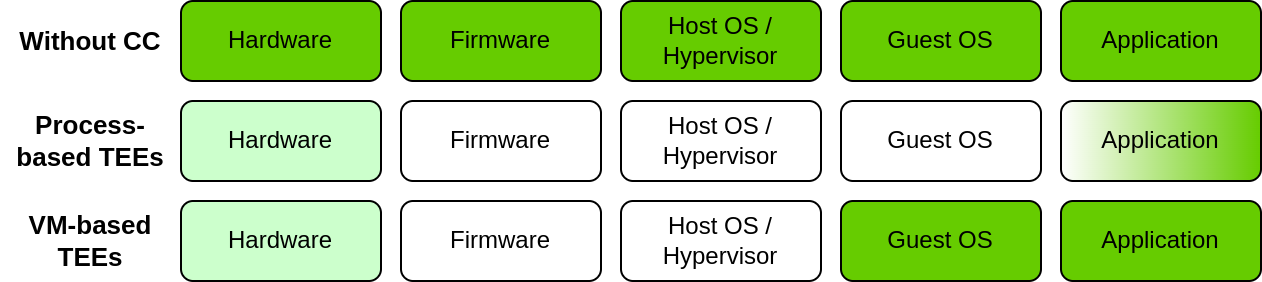
\includegraphics[width=0.85\linewidth]{resources/tee-models-comparison.drawio.png}
  \caption{Comparison of trusted execution environment models in a virtualized environment.}
  \label{figure:cc-tee-comparison}
\end{figure}

\subsection{Commercially Available TEE Technologies}
\label{sec:commercial-tee-technologies}

\begin{description}
  \item[Intel SGX]
    Intel Software Guard Extensions (SGX) provides process-based TEEs by relying
    on hardware to create enclaves that contain application code and
    confidential data. As the name implies, it is an extension of Intel's CPU
    instruction set architecture \cite{costan2016sgx}.

    The CPU protects a designated memory area called the Processor Reserved
    Memory (PRM) established by SGX, by ensuring that other software and
    hardware components, such as system software (hypervisor or OS) and DMA
    devices, do not have access to the PRM. Confidential data and application
    code of enclaves is stored in the Enclave Page Cache (EPC), which is a
    subset of the PRM. SGX relies on an untrusted system software to manage EPC
    pages by assigning EPC pages to enclaves and evicting these pages if needed.
    However, system software cannot directly access the EPC and the CPU
    maintains Enclave Page Cache Map (EPCM) in the EPC that keeps track of
    allocated EPC pages and the enclave which owns the page. Using the EPCM the
    CPU checks the correctness of the system software's allocation decisions,
    ensures that a EPC page is only assigned to a single enclave, and that only
    the assigned enclave can access and modify the EPC page. The CPU also
    encrypts EPC pages while they are stored in physical memory in order to
    prevent leaking confidential data through PME attacks and guaranteeing
    confidentiality of EPC pages after eviction.

    Initially, the system software ask the CPU to copy data from unprotected
    memory into EPC pages and assigns the pages to the enclave. After the EPC
    pages are loaded, the enclave is marked as initialized and the system
    software can not access nor modify EPC pages anymore. The CPU then measures
    SGX firmware components and the EPC pages of the enclave, producing
    attestation evidence which is then signed by the CPU using a cryptographic
    key that is only accessible by the CPU. The signature can
    then be used to verify the authenticity of the evidence, which in turn can
    be used to verify the integrity of the enclave and the SGX platform. An
    attestation can not only be requested after initialization, but also during
    runtime.

  \item[AMD SEV]
    AMD SEV-SNP is the latest iteration of AMD's Secure Encrypted Virtualization
    (SEV) technology \cite{amd2021sev, amd2017seves, amd2020sevsnp} and as the
    name implies provides VM-based TEEs.

    SEV relies on hardware embedded encryption engines that encrypt or decrypt
    memory pages written to or read from the physical memory of a machine. It
    utilizes the AMD Secure Processor (AMD-SP), which is integrated into the
    same chip as the CPU, to generate and manage cryptographic keys used for the
    en-/decryption. All software and data is tagged with an Address Space
    Identifier (ASID). The CPU uses the ASID to restrict the usage of data to
    the owner with the same ASID, and protect the data from any unauthorized
    usage. However, in the first iteration of SEV the registers of a virtual CPU
    could be used to leak confidential data when shutting down a VM.
    Subsequently, AMD released their second iteration SEV-ES (Encrypted State),
    which not only encrypted VM memory but also the virtual CPU's registers. The
    latest version SEV-SNP (Secure Nested Paging) introduced additional features
    that protect VM memory integrity.

    The attestation process for SEV VMs is similar to the attestation process of
    SGX enclaves. A hypervisor launches a VM and after the VM is fully loaded
    the VM's memory is encrypted. Subsequently, the AMD-SP measures SEV firmware
    components and VM memory pages, which are signed using a cryptographic key.
    Again, the signature can then be used for verifying the authenticity of the
    measurements, and the measurements can be used for verifying the integrity
    of the VM and the SEV platform. Attestation support in SEV and SEV-ES was
    limited, as measurements could only be requested during the launch of a VM.
    SEV-SNP supports the request of measurements at any time, enabling a more
    flexible remote attestation.
\end{description}

\subsection{Limitations}
\label{sec:limitations}

\begin{description}
  \item[Performance Impact]
    Generally, currently existing solutions either require careful configuration
    in order to achieve acceptable performance or are inappropriate for specific
    types of workloads \cite{akram2021performance}. For example due to the
    limited size of the EPC and the restricted programming model, Intel SGX
    displays a significant performance loss for high performance workloads,
    making the usage of SGX for these kinds of cases impractical.
  \item[CPU centric focus]
    Most of today's confidential computing solutions focus on a CPU-level view
    of memory permissions. This limits the application of confidential computing
    to heterogeneous computing systems, where heterogeneous accelerators are
    used in order to speed up specific computations (e.g. NPUs for machine
    learning workloads). However, there is ongoing work on integrating
    confidential computing into heterogeneous computing systems
    \cite{jiang2022cronus}.
  \item[New technology that requires further research]
    Since the introduction of Intel SGX in 2015 numerous vulnerabilities have
    been found in the SGX architecture \cite{fei2021sgxvulnerabilities}. AMD SEV
    has also not been spared, which until now required two iterations to fix the
    issues that have been discovered. Both technologies also depend on existing
    software such as hypervisors, VM firmware, and operating systems to
    implement the support of these technologies. These implementations also
    require further research and testing in order to find vulnerabilities and
    security issues.
\end{description}
